%
% File acl2018.tex
%
%% Based on the style files for ACL-2017, with some changes, which were, in turn,
%% Based on the style files for ACL-2015, with some improvements
%%  taken from the NAACL-2016 style
%% Based on the style files for ACL-2014, which were, in turn,
%% based on ACL-2013, ACL-2012, ACL-2011, ACL-2010, ACL-IJCNLP-2009,
%% EACL-2009, IJCNLP-2008...
%% Based on the style files for EACL 2006 by 
%%e.agirre@ehu.es or Sergi.Balari@uab.es
%% and that of ACL 08 by Joakim Nivre and Noah Smith

\documentclass[11pt,a4paper]{article}
\usepackage[hyperref]{acl2018}
\usepackage{times}
\usepackage{latexsym}
\usepackage{graphicx}
\usepackage{float}
\usepackage{url}

\aclfinalcopy % Uncomment this line for the final submission
%\def\aclpaperid{***} %  Enter the acl Paper ID here

%\setlength\titlebox{5cm}
% You can expand the titlebox if you need extra space
% to show all the authors. Please do not make the titlebox
% smaller than 5cm (the original size); we will check this
% in the camera-ready version and ask you to change it back.

\newcommand\BibTeX{B{\sc ib}\TeX}

\title{Language Understanding System: Final Project}

\author{Montagner Andrea - 189514\\
  {\tt andrea.montagner@studenti.unitn.it}}

\date{\today}

\begin{document}
\maketitle
\begin{abstract}
  This document contains the report of the second project of the course of Language Understanding System. The goal is to develop a simple dialog system within Rasa framework in the movie domain, which is able to interact with the user answering to pertinent questions (\textit{e.g.} director names, actors name, release year etc etc). All necessary steps will be explained, starting from the pre-processing of the data to fit the requests of Rasa, to the configuration of the database and the query system to access information. The preferred language for the both was Python (v2.7), whereas the RDBMS for the database was MySql.
\end{abstract}

\section{Introduction}

It has been almost a decade since the trend of bots' development had a sharp increase and many products were sold on the market. Even though many of them had a lot of success, one of the main issue that many both were not able to face was to recognize the context and this derives from the fact that many of them used state machine to solve this task. With the spreading of new techniques, such as machine learning algorithms, a lot of research has been done on this issue, but has not translated into actual developers tool.\\

Rasa is a framework which provides a new approach to conversational softwares: instead of taking hard-coded rules it exploits the fact that if on one hand understanding when the bot is wrong is easy, on the other hand understanding \textit{why} it is wrong can be very tricky. Following this way, it is possible to decide everything the bot can do or say, even the training can be done either in a supervised way (if data are available) or with an interactive learning starting from scratch.

\section{Data Analysis}

The provided dataset is the same of the previous project, namely the Microsoft NL-SPARQL dataset and it was already split into two parts: one for training and one for testing. In addition, each of these groups of data was divided into main data for the Movie Domain and additional features. The latter contains labels for each sentence.

To summarize, what was given were five files:
\begin{itemize}
	\item {\bfseries NL-SPARQL.train.data} containing a two columns set of data, tab separated, where the first column represent the words and the second tags,
	\item {\bfseries NLSPARQL.train.utt.labels.txt} containing a single column set of data, identifying the labels for each sentence,
	\item {\bfseries NL-SPARQL.test.data} containing a two columns set of data, tab separated, where the first column represent words and the second tags,
	\item {\bfseries NLSPARQL.test.utt.labels.txt} containing a single column set of data, identifying the labels for each sentence,
	\item {\bfseries moviedb.sql}: the database of the movie domain
\end{itemize}


\subsection{Data pre-processing}

The dataset had to be manipulated in order to be compatible with Rasa. A python script (\textit{data\_processing.py}) which takes the "raw" data in input and outputs them in a .json file in the correct format. An example of the result is shown in Figure 1.\\

\begin{figure}
	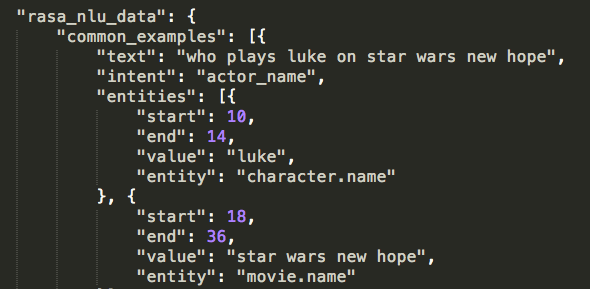
\includegraphics[scale=.7]{images/data_example}
	\caption{Example of the training data after processing}
\end{figure}

\section{Rasa-Core \&\& Rasa-NLU}

As stated before, Rasa is a framework that allows to create a complete Dialogue System, meaning training the NLU and creating the dialogue manager to handle the conversation. It is based on some concepts, that will be explained in the next subsections.

	\subsection{Texts}
	
	The text is the search query, namely the entire sentence on which the intent and the entities will be extracted.
	
	In this case, each line of the initial dataset contains a word of a sentence and the end of the sentence is delineated by an empty line. The text is a reshape of the sentence in one line.

	\subsection{Entities}
	\label{entities}
	
	An Entity consists in specific parts of the text which need to be identified. Each entity is specified with a start and end value that identify respectively the starting and the end point of the entity.
	
	In this particular case, the dataset has been provided with tagged word with IOBs, and consequently the tags are used as entity. Note that IOBs are of three type:
	\begin{itemize}
		\item [{\bfseries I}] Inside of span
		\item [{\bfseries O}] Outside of span
		\item [{\bfseries B}] Beginning of span
	\end{itemize}
	
	Only "B" and "I" tags are taken into consideration as entities, since "Outside of span" words do not bring any additional useful information. 
	
	\subsection{Intents}
	\label{intents}
	
	The intent is the intent that should be associated with the text. Basically, it is what the user is probably looking for in the sentence. 
	
	In this case, intents are taken from the label file and from some examples in the Rasa repository on Git.

	\subsection{Actions}
	\label{actions}
	
	Actions are all the things the bot can actually do. They have to follow a fixed structure, being invoked by calling the \textit{action.run()} method. Actions can do multiple things, like:
		
		\begin{itemize}
			\item Respond to a user
			\item Query a database
		\end{itemize}

	They have all to extend the \textit{Action} class, and can be of various type. The easiest are called UtterActions, which just send a message to the user. There is also the possibility of creating custom, more complex actions which perform composite commands/queries. 
	
	Custom actions are implemented in \textit{actions.py}
	
	\subsection{Domain}
		Finally, the last crucial component is the domain, which defines the universe in which the bot operates. It is a \textit{.yml} file, which contains:
		\begin{itemize}
			\item Slots
			\item Entities (\ref{entities})
			\item Intents ((\ref{intents})
			\item Templates 
			\item Actions (\ref{actions})
		\end{itemize}

where slots contain what the bot needs to keep track during the conversation, entities, intents and actions are exactly what is explained few subsection above, and templates represent answers to the basic actions, like initial/final greetings, negative result to search and so on.

The domain file is \textit{domain.yml}.
	
\section{Database}
 
	\subsection{MySql}
	
	As far as the database part is concerned, it is pretty simple and straightforward. MySql has been used as RDBMS because it is well interfaced with Python through toolkit like SQLAlchemy \cite{SQLA}.
	For this project the file \textit{moviedb.sql} has been loaded into MySql in order to be accessible to queries. It is composed by 2 tables, Movie and Movies, of which only movie has been used. Structure of the table is shown in Figure 2
	
	\begin{figure*}
		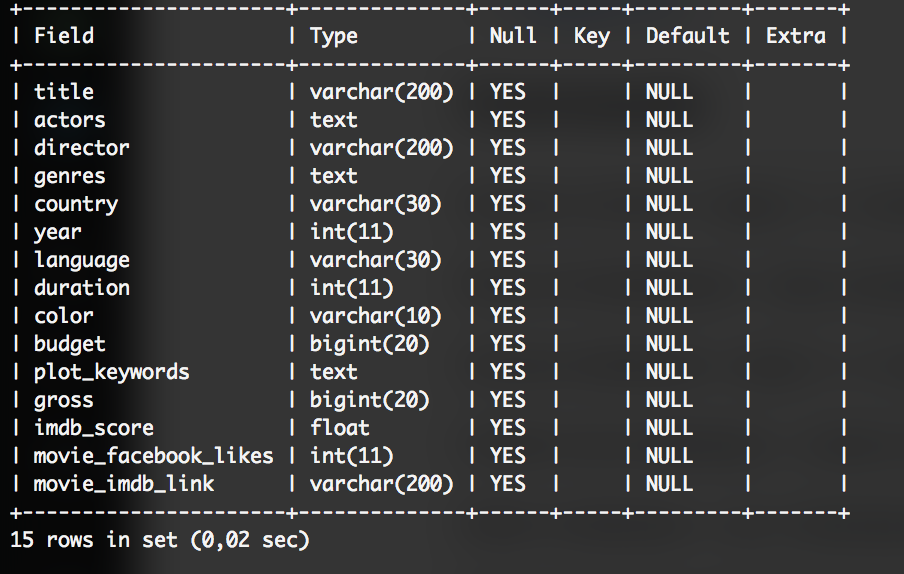
\includegraphics[width=\textwidth]{images/database}
		\center\caption{'Movie' table of the database}
	\end{figure*}
	
	\subsection{Accessing}
	
	In order to access the database and make queries to obtain information, it has been used a Python access tool, named SQLSoup \cite{SQLS}, which is built on top of SQLAlchemy. An issue when thinking about how to search the database was the fact that target users are very different from each other and can make grammar mistakes in searching information. To solve this problem the \textit{ilike} function has been used, which is the correspondent of the \textit{LIKE} operator of the SQL language, in order to collect all similar matches to the research. The only cons this solution has, is that there is the necessity of another function which finds the best match between the one returned from the search.
	
	The implementation of the database manager can be found in \textit{db\_manager.py}.

\section{Bot}

The bot is implemented in \textit{bot.py} and its structure is very simple, it let the user decide in which way to run depending on the input parameter:\\

	\begin{itemize}
		\item {\bfseries train-nlu}
		
			This is the first step to be done, it takes as inputs the training data and the domain file, then it trains a Trainer over the data and stores the result in a directory.
		\item {\bfseries train-dialogue}
		
			After training the NLU, it is ready for the question/answer phase, but it does not know how to handle the conversation. For this purpose, a dialogue manager (DM) is trained passing as input the NLU previously created, the policies (Keras and Memoization in this case). the DM is trained over a data file, here identified as \textit{stories.md}, which contains examples of conversation in order to help to understand the flow.
			There is also the passobility of an "online\_training", that is exactly the one previously referenced as \textit{interactive learning} when describing Rasa. In this way, it is possible to train the agent step by step, immediately correcting its answers when wrong.
		\item {\bfseries run}
	
			Standard way to run the bot, once both training are done.
	\end{itemize}

\section{Training and evaluation}

NLU has been trained using Rasa standard evaluation method (\textit{python -m rasa\_nlu.evaluate}) and results are above $90\%$ for all criterions: F1 score, precision. accuracy.

\begin{figure}[h]
	\center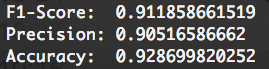
\includegraphics[scale=1.4]{images/evaluation}
	\center\caption{Results of evaluation of the NLU}
\end{figure}

When running the second step, though, I faced an big issue. Whenever I tried to access the database I got the following error:

\begin{figure}[h]
	
\includegraphics[scale=.55]{images/error}
\end{figure}

This error is shown because a \textit{MySQLdb} module is missing. As a consequence I can not access the database from Python, meaning I am not able to retrieve any information from it. I tried to solve this problem in many ways, from the less destructive ones (\textit{e.g.} try to reinstall pip) to the more destructive ones (\textit{e.g.} install via sudo pip, delete and reinstall Python) but none of these have worked. 

For this reason, I can not train the dialogue manager neither with the supervised training nor with the online, interactive learning. I am currently searching a way to solve it, in order to do  , even if very late.

\begin{figure}[h]
	\center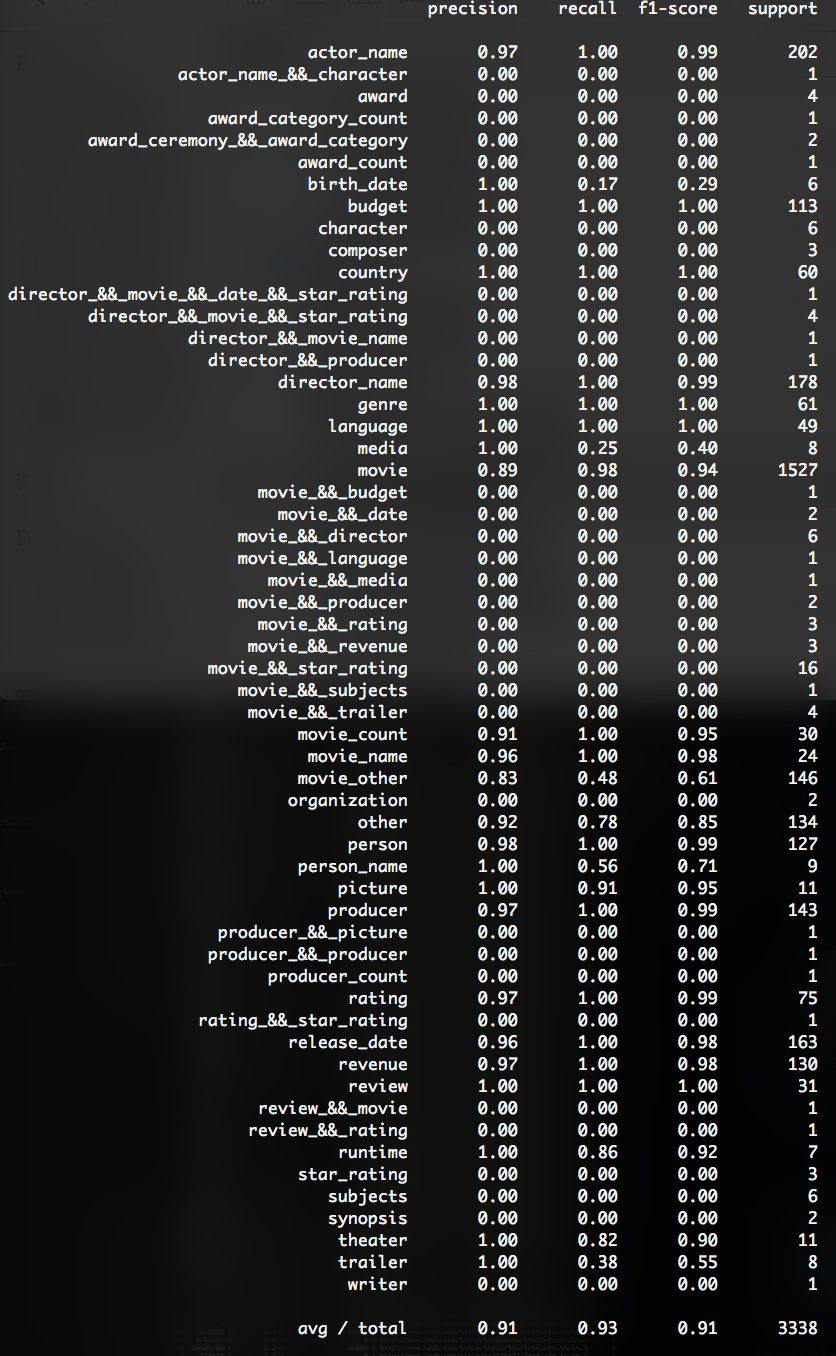
\includegraphics[scale=.5]{images/results}
	\center\caption{Classification report of NLU training with Rasa}
\end{figure}

\section{Conclusions}

In this project a chat-bot implementation within Rasa framework is shown, even if with some limitations. It is possible indeed to train the NLU with satisfactory results (above $90\%$ of F1) as shown above, but it is not possible to train the dialogue manager due to an error I am not able to solve.\\

Even though, the pipeline of the implementation follows the one provided in the example in the GitHub repository with some insight from the official documentation of Rasa, the error is just a matter of the machine, which for some reason refuses to install some modules.

\end{document}
